\documentclass[12pt]{amsart}
\usepackage{amsaddr}
\usepackage{marktext} 
%% Remove draft for real article, put twocolumn for two columns
\usepackage{svmacro}
\usepackage[utf8]{inputenc}
\usepackage{lineno}
\usepackage[style=alphabetic, backend=biber]{biblatex}
\addbibresource{bibliography.bib}

%% commentary bubble
\newcommand{\SV}[2][]{\sidenote[colback=green!10]{\textbf{SV\xspace #1:} #2}}

%% Title 
\title{ MATH 102: Ideas  of Math }
\author{ Worksheet 8 }

\date{Nov 1, 2023}

\begin{document}

\maketitle

\section{Concepts}

     \begin{definition}[Newstead, Chapter 4]
    A function $f$ from a set $X$ to a set $Y$ is a specification of elements 
    $f(x) \in Y$ for $x\in X$ such that
    \begin{equation*}
        \forall x \in X, \exists! y \in Y, y = f(x) \,.
    \end{equation*}
    Given $x\in X$, the unique element $f(x)\in Y$ is called the value of $f$ at $x$.

    $X$ is called the \emph{domain} of $f$, and $Y$ is called the \emph{codomain}.

    We denote the \emph{range} of $f$ is
    \begin{equation*}
        f(X) = \set{ f(x) \st x \in X} \,.
    \end{equation*}

    We write $f:X\to Y$ to denote the assertion that $f$ is a function with domain $X$ and codomain $Y$.

    We sometimes write $\Dom(f)$ to mean domain of $f$
    and $\Ran(f)$ to mean the range of $f$.
    \end{definition}


    \begin{definition}
    Let $X, Y$ be sets. The \emph{cartesian product} of $X$ and $Y$ is the set $X\times Y$, defined by 
    \begin{equation*}
        X\times Y = \left\{ (a,b) \vert a\in X \wedge b \in Y  \right\} \,.
    \end{equation*}
    The elements $(a,b) \in X\times Y$ are called \emph{ordered pairs}, whose defining property is that
    \begin{equation*}
        \forall x\in X, \forall y \in Y, (a,b) = (x,y) \iff a = x \wedge b = y \,.
    \end{equation*}
    \end{definition}


    \begin{definition}
    Let $f: X\to Y$ be a function. 
    The \emph{graph} of $f$ is the subset $\Gr(f) \subseteq X \times Y$ defined by
    \begin{equation*}
        \Gr(f) = \set{ (x,f(x)) | x \in X   }
        = 
        \set{ (x,y) \in X \times Y | y = f(x)} \,.
    \end{equation*}
    \end{definition}



    \begin{definition}
        Let $A, B$ be sets. Then the set $R \subseteq A \times B$ is called a relation from $A$ to $B$.

        We also define the domain and range of a relation $R$.

        \begin{gather*}
            \Dom(R) = \set{a \in A \st \exists b \in B, (a,b) \in R}  \\
            \Ran(R) = \set{ b\in B \st \exists a \in A, (a,b) \in R } \,.
        \end{gather*}

        If $(x,y) \in R$, then we say that $x$ is related to $y$ by $R$ and write $x R y$.
    \end{definition}

\section{Problems}
\begin{problem}
    The two concepts of relation and logical predicate are closely related (no pun intended). Can you make this connection?
\end{problem}

\begin{problem}
Let $R$ be a relation so that $x R y$ means ``there is an arrow from $x$ to $y$''.

Consider the following pictures and specify in each case
\begin{enumerate}
    \item what is $R$?
    \item what is $\Dom(R)$?
    \item what is $\Ran(R)$?
\end{enumerate}
    \begin{figure}[h!]
        \begin{center}
            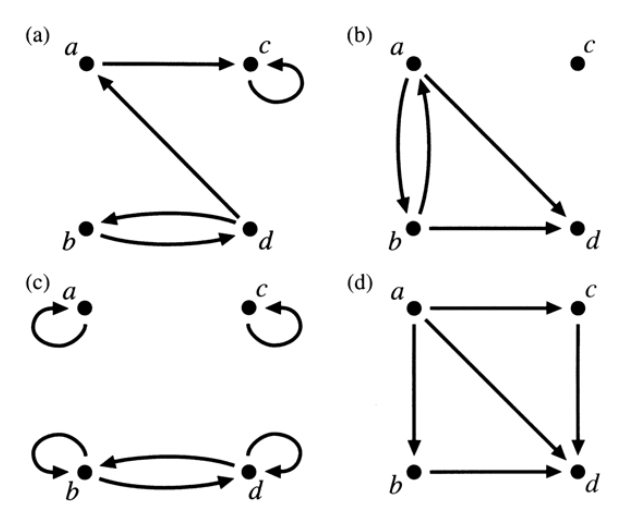
\includegraphics[width=0.95\textwidth]{graph}
        \end{center}
    \end{figure}
\end{problem}

\begin{problem}
    The two concepts functions and relations are closely related.
    In fact, one of the standard ways to define a function is as follows.

    
    \begin{definition}[Alternative Definition of Functions, Velleman Chapter 5]
        Suppose $F$ is a relation from $A$ to $B$. Then $F$ is called a function from $A$ to $B$ if for every $a \in A$ there is exactly one $b \in B$ such that $(a, b) \in F$. In other words, to say that $F$ is a function from $A$ to $B$ means:
\[
\forall a \in A \, \exists! b \in B \, ((a, b) \in F).
\]

To indicate that $F$ is a function from $A$ to $B$, we will write $F : A \to B$.
    \end{definition}

    How are the two definitions related? What is the difference?
\end{problem}


\end{document}
